\documentclass[12pt,draftcls,onecolumn]{IEEEtran}  % Comment this line out if you need a4paper

%\documentclass[a4paper, 10pt, conference]{ieeeconf}      % Use this line for a4 paper


\usepackage{cite}
\usepackage{epsfig}
\usepackage{epstopdf}
\usepackage[cmex10]{amsmath}
\usepackage{amssymb}
\usepackage{array}
\usepackage{mdwmath}
\usepackage{mdwtab}
\usepackage{cases}
\usepackage{eqparbox}
\usepackage{subfig}
\usepackage{color}
\usepackage{pifont}
\usepackage{tikz}
\definecolor{brown}{rgb}{0.823529 ,0.411765, 0.117647}
%\usepackage[usenames,dvipsnames]{color}
%\usepackage{ulem}

\IEEEoverridecommandlockouts
% This command is only needed if% you want to use the \thanks command

\overrideIEEEmargins                                      % Needed to meet printer requirements.

% See the \addtolength command later in the file to balance the column lengths
% on the last page of the document

% The following packages can be found on http:\\www.ctan.org
%\usepackage{graphics} % for pdf, bitmapped graphics files
%\usepackage{epsfig} % for postscript graphics files
%\usepackage{mathptmx} % assumes new font selection scheme installed
%\usepackage{times} % assumes new font selection scheme installed
%\usepackage{amsmath} % assumes amsmath package installed
%\usepackage{amssymb}  % assumes amsmath package installed

%\title{\LARGE \bf
%Distributed $\varepsilon$-Nash Strategies for Multi-Agent Formation Control}
%
%
%\author{Wei~Lin$^\dag$,~\IEEEmembership{Student Member,~IEEE,}
%        Zhihua~Qu$^\dag$,~\IEEEmembership{Fellow,~IEEE,}
%        and~Marwan~A. Simaan$^\dag$,~\IEEEmembership{Life Fellow,~IEEE}
%% <-this % stops a space
%\thanks{*This work is supported in part by US National Science Foundation under grants ECCS-1308928 and CCF-0956501 as well as by US Department of Energy's award DE-EE0006340 under the Grid Engineering for Accelerated Renewable Energy Deployment (GEARED) program and another subcontract under the Solar Energy Grid Integration Systems (SEGIS) program (phases I to III).}% <-this % stops a space
%\thanks{$^\dag$Wei Lin, Zhihua Qu, and Marwan A. Simaan are with the Department of EECS, University of Central Florida, Orlando, Florida, 32816, USA. Emails:
%        {\tt\small weilin0929@gmail.com, qu@eecs.ucf.edu, simaan@eecs.ucf.edu}.}%
%%
%}

\begin{document}
\title{\LARGE \bf
Distributed Game Strategy Design with Application to Multi-Agent Formation Control}


\author{Wei~Lin,~\IEEEmembership{Member,~IEEE,}
        Zhihua~Qu~\IEEEmembership{Fellow,~IEEE,},~and
        Marwan~A. Simaan,~\IEEEmembership{Life Fellow,~IEEE}
% <-this % stops a space
\thanks{This work is supported in part by US National Science Foundation under grants ECCS-1308928 and CCF-0956501, by US Department of Energy¡¯s award DE-EE0006340, by US Department of Transportation¡¯s award DTRT13-G-UTC51, by L-3 Communication¡¯s contract 11013I2034, and by Leidos¡¯ contract P010161530.}% <-this % stops a space
\thanks{Wei Lin is with Western Digital Corporation, Irvine, CA, 92612, USA. E-mail: weilin0929@gmail.com.}
\thanks{Zhihua Qu and Marwan A. Simaan are with the Department of EECS, University of Central Florida, Orlando, Florida, 32816, USA, e-mails: qu@eecs.ucf.edu, simaan@eecs.ucf.edu.}%
%
}


%\markboth{Journal of \LaTeX\ Class Files,~Vol.~11, No.~4, December~2012}%
%{Shell \MakeLowercase{\textit{et al.}}: Bare Demo of IEEEtran.cls for Journals}

\maketitle

\IEEEpeerreviewmaketitle

%%%%%%%%%%%%%%%%%%%%%%%%%%%%%%%%%%%%%%%%%%%%%%%%%%%%%%%%%%%%%%%%%%%%%%%%%%%%%%%%
\begin{abstract}
In this paper, we consider {a} multi-agent formation control problem from {a} game {theory} point of view. It is well known that a major difficulty in a communication network based formation control problem is that each agent is only able to exchange information {with other agents} according to the communication topology. This information constraint prevents many game strategy design approaches that require individual agents to have global information from being implemented in many cases. We formulate the formation control problem {in such a way that individual agents try to minimize their locally measured formation errors and {to} solve it as a differential game problem}. We consider two cases of non-cooperative and cooperative games and {propose} a novel distributed design approach that utilizes the relationship between the initial and terminal state variables. This approach is applied to an illustrative formation control example among three agents and the formation errors under various scenarios are compared and analyzed.
\end{abstract}

\newtheorem{Def}{Definition}
\newtheorem{Asu}{Assumption}
\newtheorem{thm}{Theorem}
\newtheorem{Pro}{Proposition}
\newtheorem{Alg}{Algorithm}
\newtheorem{Lem}{Lemma}
\newtheorem{Rmk}{Remark}
\newtheorem{Cor}{Corollary}

\section{Introduction}
{An} important application of cooperative control theory \cite{ren,Qu} {is} the multi-agent formation control problems \cite{Stipanovic2004,Keviczky2008,JiananWang2012}. {This problem revolves around designing} local information constrained control inputs for the agents (mobile robots, unmanned vehicles, etc) and {making} their positions {follow} a prescribed formation. There {is considerable work} done in this field and the comprehensive review paper \cite{Cao2013} on multi-agent distributed control systems is a good reference on {recent} progress {in} cooperative control theory including the formation control problem. Recently, multiple attempts \cite{anderson1998formation,DongbingGu2008,SemsarKazerooni20092205} have been made to incorporate {differential} game theory \cite{Isaacs,Basar} into the formation control design problem. {A fundamental connection {between these two problems} can be explained as follows: in a multi-agent formation control problem, all the agents are basically trying to minimize the formation errors between each other. If every agent is able to observe all the other agents, then the problem can be essentially viewed as an optimal control problem where a common performance index of global formation errors can be assigned for all the agents. However, in most of {realistic} applications,} since the agents are usually connected through {a} communication network {with} a certain topology, they are only able to exchange information with each other in a distributed manner (i.e., to share information locally). {In {this} case, instead of minimizing a globally defined performance index, it is {more realistic} for each agent to only minimize a performance index of its locally measured formation errors. This scenario is exactly equivalent to that of a differential game where each player is trying to minimize its own performance index. Therefore, most {multi-agent} formation control design {problems} can be viewed and solved as {differential game problems}. The game solutions including {Nash equilibria} for non-cooperative agents and Pareto optimality for cooperative agents can {be} well established. However, solving {for} the Nash and Pareto solutions under distributed information is not a trivial task in the multi-agent environment because of the following two {issues}: (1) the strategy for each agent has to conform to its local information topology constraint and (2) local strategy computing within each agent is preferred rather than centralized strategy computing where strategies are designed by a centralized designer and assigned to individual agents.} In \cite{DongbingGu2008,SemsarKazerooni20092205}, the first {issue} has been addressed and the corresponding Nash and Pareto strategies are considered for the formation control problem as a differential game. {In} this present paper, we will focus more on the second aspect. By investigating the structure of the game solution in more details, a strategy design approach as well as {an} implementation algorithm {are} proposed for each agent to carry out its optimal control strategy design in a fully distributed manner. The {remainder} of this paper is organized as follows. A brief setup of the game {problem} is presented in Section \ref{setup}. The main results of the distributed Nash and Pareto strategy {designs} are presented in Section \ref{mainresult1} and \ref{mainresult2} {respectively}. An illustrative example with three agents under noncooperative and cooperative cases is presented and analyzed in Section \ref{simulation}.


%%%%%%%%%%%%%%%%%%%%%%%%%%%%%%%%%%%%%%%%%%%%%%%%%%%%%%%%%%%%%%%%%%%%%%%%%%%%%%%%
\section{Problem Formulation}\label{setup}
We consider the {finite-time} formation control problem between $N$ agents in the $n$-dimensional Euclidean space where the motion dynamics of each agent is described as the following double integrator model:
\begin{equation}
\begin{bmatrix}
\dot{p}_i\\ \dot{v}_i
\end{bmatrix}=\begin{bmatrix}
0&I_n\\0&0
\end{bmatrix}\begin{bmatrix}
p_i\\
v_i\end{bmatrix}+\begin{bmatrix}
0\\ I_n
\end{bmatrix}u_i\label{systemxi}
\end{equation}
for $i=1,\cdots,N$. {Vector $p_i\in\mathbb{R}^n$ and $v_i\in\mathbb{R}^n$ are the position and velocity of agent $i$ respectively.} Vector $u_i\in\mathbb{R}^{n}$ is the acceleration control of agent $i$. We assume that the agents are able to exchange information with each other through a communication network {whose topology can be described by a set $\mathcal{E}$ in graph theory. An edge $e_{ij}\in\mathcal{E}$ represents information being transmitted from agent $j$ to agent $i$}. The objective of the agents is to form a prescribed formation over a finite time interval, which is equivalent to individual agents minimizing the following performance indices:

Since every agent is only aware of its local communication pattern and its own performance index, this formation problem can be regarded as a differential game problem where each player {has} its own objectives to pursue over a time interval. In this paper, we consider two types of open-loop {(where the control inputs are functions of initial states and time only)} formation control approaches through {differential} game strategy design. Specifically, {if the control inputs $u_1,\cdots,u_N$ can be looked as strategies}, then for the formulated problem, strategies {$u^{N}_{1},\cdots,u^{N}_N$} are the Nash strategies and form a Nash equilibrium if the inequality
\begin{align}
&{J_{i}(u_1^{N},\cdots,u^{N}_i,\cdots,u^{N}_N)\leq J_{i}(u_1^{N},\cdots,u_i,\cdots,u^{N}_N)}\label{Nashinequality}
\end{align}
holds for all $u_i\in U_i$ and for all $i=1,\cdots,N$, where $U_i$ is the open-loop control set for agent $i$. The Nash equilibrium is an equilibrium where it is not possible for any agent to lower its performance index value by unilaterally deviating from its Nash strategy. The Nash equilibrium is a widely used solution in the situation where the players do not {cooperate} with each other. On the other hand, The strategies $u^{P}_0,u^{P}_{1},\cdots,u^{P}_N$ are the Pareto strategies and {form a Pareto optimality if the inequality
\begin{align}
&J_{i}(u^P_1,\cdots,u^P_N)< J_{i}(u_1,\cdots,u_N) \label{inequality}
\end{align}
holds for at least one $i\in\{1,\cdots,N\}$.} The Pareto optimality can be interpreted as a solution in which any changes made do not help lower every agent's performance index value. The Pareto optimality is a widely used solution in the situation where the players can {cooperate} with each other. In the following sections, two formation control approaches will be proposed based on the open-loop Nash strategy (assuming that the agents do not {cooperate}) and the open-loop Pareto strategy (assuming that the agents {cooperate}).

%%%%%%%%%%%%%%%%%%%%%%%%%%%%%%%%%%%%%%%%%%%%%%%%%%%%%%%%
\section{Free Terminal State}
If we let the terminal state be free, the performance indices are
\begin{align}
J_i=&\sum_{e_{ij}\in\mathcal{E}} \frac{1}{2}\bigg[\|p_i(t_f)\|^2+\|p_i(t_f)-p_j(t_f)-\mu_{ij}\|^2+ +\|v_i(t_f)\|^2+\|v_i(t_f)-v_j(t_f)\|^2\bigg]\notag\\
&+\frac{1}{2}\int^{t_f}_0 \|u_i\|^2  \mbox{d}t\label{JiFormation}
\end{align}
for $i=1,\cdots,N$, where $\|\cdot\|$ is the Euclidean norm, $\mu_{ij}$ is the desired displacement vector pointing from {agent} $j$ to {agent} $i$, and $r_i$ is a positive scalar. {Minimizing performance index $J_i$ means that every agent will try to minimize its locally measured total terminal formation error and terminal velocity error according to the graph while at the same time minimizing its control effort during the time interval.
\begin{thm}[Free Terminal State]
For the $N$-agent linear quadratic differential game of fixed duration $[0,t_f]$ defined by agents' dynamics (\ref{systemxi}) and performance indices (\ref{JiFormation}), if the information structure of every agent is open-loop, i.e., $U_i=\{u_i(t,p_0,v_0)\in \mathbf{R} \mid t\in[0,t_f]\}$, there exists a unique Nash equilibrium and corresponding open-loop control strategies are
\begin{align}
&u^*(t,p_0,v_0)\notag\\
&=
\begin{bmatrix}
(t-t_f)L&-L
\end{bmatrix}
\begin{bmatrix}
I-\frac{1}{6}t_f^3L&-t_fI-\frac{1}{2}t_f^2L\\
\frac{1}{2}t_f^2L&I+t_fL
\end{bmatrix}^{-1}\left(
\begin{bmatrix}
p_0\\
v_0
\end{bmatrix}+\begin{bmatrix}
-\frac{1}{6}t_f^3I\\ \frac{1}{2}t_f^2I
\end{bmatrix}\mu\right)
+
(t_f-t)\mu\label{uNash}
\end{align}
in vector form, where
\[u_i=\begin{bmatrix}
u_1 \\ \cdots \\ u_N
\end{bmatrix},\quad
p=\begin{bmatrix}
p_1\\ \cdots\\ p_N
\end{bmatrix},\quad
v=\begin{bmatrix}
v_1\\ \cdots\\v_N
\end{bmatrix},\quad \mu=\begin{bmatrix}
\sum_{e_{1j}\in{\mathcal{E}}}\mu_{1j}\\
\cdots\\
\sum_{e_{Nj}\in{\mathcal{E}}}\mu_{Nj}
\end{bmatrix},\]
and matrix $L=[l_{ij}]\in\mathbb{R}^{N\times N}$ is the graph Laplacian matrix defined by
\begin{equation}
l_{ij}=\left\{\begin{array}{ll}
-1&\mbox{if $e_{ij}\in\mathcal{E}$ for $j\neq i$}\\
0&\mbox{if $e_{ij}\notin\mathcal{E}$ for $j\neq i$}\\
\displaystyle -\sum^N_{q=1,q\neq i}l_{iq}&\mbox{if $j=i$}
\end{array}\right..\label{laplacian}
\end{equation}
\end{thm}

\begin{proof}
We define the Hamiltonian for agent $i$ as
\begin{align}
H_i=&\frac{1}{2}\|u_i\|^2+ \lambda_{pi}^Tv_i+
\lambda_{vi}^Tu_i
\end{align}
where vectors $\lambda_{pi}$ and $\lambda_{vi}$ are the Lagrangian multipliers. Necessary conditions for the existence of open-loop Nash equilibria are
\begin{subequations}\begin{align}
&\dot{p}_{i}=\frac{\partial H_i}{\partial \lambda_{pi}}=v_i,\label{NecPi}\\ &\dot{v}_{i}=\frac{\partial H_i}{\partial \lambda_{vi}}=u_i\label{NecPi1}\\
&\dot{\lambda}_{pi}=-\frac{\partial H_i}{\partial p_{i}}= 0,\\
&\dot{\lambda}_{vi}=-\frac{\partial H_i}{\partial v_{i}}= -\lambda_{pi},\label{NecPi2}\\
&\lambda_{pi}(t_f)= \sum_{e_{ij}\in\mathcal{E}}[p_{i}(t_f)-p_{j}(t_f)-\mu_{ij}],\label{NecPi3}\\
&\lambda_{vi}(t_f)= \sum_{e_{ij}\in\mathcal{E}}[v_{i}(t_f)-v_{j}(t_f)],\label{NecPi4}\\
&\frac{\partial H_i}{\partial u_i}=u_i+\lambda_{vi} =0,\label{NacU}
\end{align}
\end{subequations}
for all $i=1,\cdots,N$. Therefore, the existence of the Nash equilibria is equivalent to the solvability of above equations given initial states $p_i(0)$ and $v_i(0)$ for all $i=1,\cdots,N$. The uniqueness of the Nash equilibrium is equivalent to the uniqueness of the solution. From (\ref{NacU}), the control vector can be obtained as
\begin{align}
u(t)=-\lambda_{v}(t),\label{ulambda}
\end{align}
where $u=[u_1,\cdots,u_N]^T$ and $\lambda_v=[\lambda_{v1},\cdots,\lambda_{vN}]^T$.
Denoting $\lambda_p=[\lambda_{p1},\cdots,\lambda_{pN}]^T$, state and co-state equations (\ref{NecPi})-(\ref{NecPi2}) can be expressed compactly as
\begin{align*}
\begin{bmatrix}
\dot{p}\\
\dot{v}\\
\dot{\lambda}_{p}\\
\dot{\lambda}_{v}
\end{bmatrix}=\begin{bmatrix}
0&I&0&0\\
0&0&0&-I\\
0&0&0&0\\
0&0&-I&0
\end{bmatrix}\begin{bmatrix}
p\\
v\\
\lambda_{p}\\
\lambda_{v}
\end{bmatrix}
\end{align*}
The solution to above first order differential equation is
\begin{align}
\begin{bmatrix}
p(t)\\
v(t)\\
\lambda_{p}(t)\\
\lambda_v(t)
\end{bmatrix}=\begin{bmatrix}
I&t I&1/6t^3&-1/2t^2I\\
0&I&1/2t^2I&-t I\\
0&0&I&0\\
0&0&-t I&I
\end{bmatrix}\begin{bmatrix}
p_0\\
v_0\\
\lambda_{p}(0)\\
\lambda_{v}(0)
\end{bmatrix}\label{twopointODE}
\end{align}
for $t\in[0,t_f]$. The control vector (\ref{ulambda}) can be now expressed as
\begin{align}
u=\begin{bmatrix}
tI& -I
\end{bmatrix}\begin{bmatrix}
\lambda_{p}(0)\\
\lambda_{v}(0)
\end{bmatrix}. \label{ulamdapv}
\end{align}
From (\ref{NecPi3})-(\ref{NecPi4}), we have
\begin{align}
\begin{bmatrix}
p(t_f)\\
v(t_f)\\
\lambda_{p}(t_f)\\
\lambda_v(t_f)
\end{bmatrix}=\begin{bmatrix}
I&0\\
0&I\\
L&0\\
0&L
\end{bmatrix}\begin{bmatrix}
p(t_f)\\
v(t_f)
\end{bmatrix}-\begin{bmatrix}
0\\0\\I\\0
\end{bmatrix}\mu\label{p0pf}.
\end{align}
Substituting $t=t_f$ and (\ref{p0pf}) into (\ref{twopointODE}) yields
\begin{align}
\begin{bmatrix}
p_0\\
v_0\\
\lambda_{p}(0)\\
\lambda_{v}(0)
\end{bmatrix}=&\begin{bmatrix}
I-\frac{1}{6}t_f^3L&-t_fI-\frac{1}{2}t_f^2L\\
\frac{1}{2}t_f^2L&I+t_fL\\
L&0\\
t_fL&L
\end{bmatrix}\begin{bmatrix}
p(t_f)\\
v(t_f)
\end{bmatrix}-\begin{bmatrix}
-\frac{1}{6}t_f^3\\ \frac{1}{2}t_f^2I \\I\\ t_fI
\end{bmatrix}\mu\label{p0lambdapf}
\end{align}
The control vector (\ref{ulamdapv}) can be further expressed as
\begin{align}
u=\begin{bmatrix}
(t-t_f)L&-L
\end{bmatrix}\begin{bmatrix}
p(t_f)\\
v(t_f)
\end{bmatrix}
+
(t_f-t)\mu. \label{utf}
\end{align}
From (\ref{p0lambdapf}), the relationship between $[p_0,v_0]^T$ and $[p(t_f),v(t_f)]^T$ can be obtained as
\begin{align}
\begin{bmatrix}
p_0\\
v_0
\end{bmatrix}=\begin{bmatrix}
I-\frac{1}{6}t_f^3L&-t_fI-\frac{1}{2}t_f^2L\\
\frac{1}{2}t_f^2L&I+t_fL
\end{bmatrix}
\begin{bmatrix}
p(t_f)\\
v(t_f)
\end{bmatrix}-\begin{bmatrix}
-\frac{1}{6}t_f^3I\\ \frac{1}{2}t_f^2I
\end{bmatrix}\mu,\label{p0pf}
\end{align}
which can be rewritten as
\begin{align}
\begin{bmatrix}
p(t_f)\\
v(t_f)
\end{bmatrix}=\begin{bmatrix}
I-\frac{1}{6}t_f^3L&-t_fI-\frac{1}{2}t_f^2L\\
\frac{1}{2}t_f^2L&I+t_fL
\end{bmatrix}^{-1}\left(
\begin{bmatrix}
p_0\\
v_0
\end{bmatrix}+\begin{bmatrix}
-\frac{1}{6}t_f^3\\ \frac{1}{2}t_f^2I
\end{bmatrix}\mu\right)\label{pfp0}.
\end{align}
The above matrix is invertible because it is product of two invertible matrices as shown below
\begin{align}
\begin{bmatrix}
I-\frac{1}{6}t_f^3&-t_fI-\frac{1}{2}t_f^2L\\
\frac{1}{2}t_f^2L&I+t_fL
\end{bmatrix}=\begin{bmatrix}
I&-t_fI\\
0&I
\end{bmatrix}\left(I+W\otimes L\right),\label{matrixdecompose}
\end{align}
where $\otimes$ is Kronecker product,
\begin{align}
&W=\begin{bmatrix}
t_f^3/3I&t_f^2/2I\\
t_f^2/2I&t_fI
\end{bmatrix}\label{W},
\end{align}
and Laplacian matrix $L$ is known to be positive semi-definite. Substituting (\ref{pfp0}) into (\ref{utf}) yields (\ref{uNash}). Therefore, the open-loop Nash equilibrium exists and is unique.
\end{proof}

\begin{Rmk}
One might be interested in the limiting case of open-loop Nash equilibrium. The resulting control trajectory will be the same as the one for closed-loop Nash equilibrium under no state disturbance such that system is asymptotically stable.
\end{Rmk}

As we have mentioned, since each agent is only aware of its own performance index and its local communication topology, computing and implementing open-loop Nash strategy (\ref{uNash}) conflict with such constraints. In fact, we are able to overcome this difficulty by carrying out distributed state estimation. Specifically, we let all agents exchange certain information across the communication network to estimate terminal variable values in a distributed manner. Toward that, the following theorem is propose.
\begin{thm}\label{Thm1}
If agent $i$ updates its estimation vectors $\hat{p}_i$ and $\hat{v}_i$ in a distributed manner according to
\begin{align}
\begin{bmatrix}
\dot{\hat{p}}_i\\
\dot{\hat{v}}_i
\end{bmatrix}=&g_i\left\{\begin{bmatrix}
p_i(0)\\
v_{i}(0)
\end{bmatrix}+\frac{1}{r_i}\begin{bmatrix}
(t_f^3/3)\mu_i\\
(t_f^2/2)\mu_i
\end{bmatrix}-\begin{bmatrix}
\hat{p}_i\\
\hat{v}_i
\end{bmatrix}-\frac{1}{r_i}W\sum_{e_{ij}\in\mathcal{E}}\left(\begin{bmatrix}
\hat{p}_i\\
\hat{v}_i
\end{bmatrix}-\begin{bmatrix}
\hat{p}_j\\
\hat{v}_j
\end{bmatrix}\right)\right\},\label{update}
\end{align}
where $g_i$ is a positive scalar, then
\begin{equation}
\lim_{\tau\rightarrow\infty}\begin{bmatrix}
\hat{p}_i(\tau)\\
\hat{v}_i(\tau)
\end{bmatrix}=\begin{bmatrix}
p_i(t_f)\\
v_i(t_f)
\end{bmatrix}
\label{limit}
\end{equation}
for $i=1,\cdots,N$, where $p_i(t_f)$ and $v_i(t_f)$ are the terminal variables specified in (\ref{pfp0}) under open-loop Nash strategy vector (\ref{uNash}).
\end{thm}
\begin{proof}
Firstly, under open-loop Nash strategies (\ref{uNash}), the relationship between initial state and terminal state is given by (\ref{p0pf}). Substituting (\ref{matrixdecompose}) yields
\begin{equation}
\begin{bmatrix}
I&t_fI\\
0&I
\end{bmatrix}\begin{bmatrix}
p(0)\\
v(0)
\end{bmatrix}=M\begin{bmatrix}
p(t_f)\\
v(t_f)
\end{bmatrix}-\begin{bmatrix}
(t_f^3/3)(R^{-1}\otimes I_n)\\
(t_f^2/2)(R^{-1}\otimes I_n)
\end{bmatrix}\mu\label{sf}
\end{equation}
where $R=\mbox{diag}\{r_1,\cdots,r_N\}$ and
\begin{equation}
M=I+W\otimes (R^{-1}L),\label{M}
\end{equation}
Since all the eigenvalues of a Laplacian matrix have nonnegative real parts, all the eigenvalues of matrix $M$ in (\ref{M}) have positive real parts and matrix $M$ is hence invertible. Secondly, combining equations (\ref{update}) for $i=1,\cdots,N$ in a more compact vector form yields
\begin{align}
\begin{bmatrix}
\dot{\hat{p}}\\
\dot{\hat{v}}
\end{bmatrix}=&G\left(\begin{bmatrix}
p(0)+t_fv(0)\\
v(0)
\end{bmatrix}-M\begin{bmatrix}
\hat{p}\\
\hat{v}
\end{bmatrix}+\begin{bmatrix}
(t_f^3/3)(R^{-1}\otimes I_n)\\
(t_f^2/2)(R^{-1}\otimes I_n)
\end{bmatrix}\mu\right),\label{stacked}
\end{align}
where $\hat{p}=[\hat{p}_1^T\;\cdots \hat{p}_N^T]^T$, $\hat{v}=[\hat{v}_1^T\;\cdots \hat{v}_N^T]^T$, {$G=\mbox{blkdiag}\{g_1I,\cdots,g_NI\}$}. Since all the eigenvalues of matrix $M$ has positive real parts, system (\ref{stacked}) is asymptotically stable and final convergent values of $\hat{p}$ and $\hat{v}$ are identical to $p(t_f)$ and $v(t_f)$ in equation (\ref{pfp0}). Therefore, equation (\ref{limit}) holds for all $i=1,\cdots,N$.
\end{proof}

\section{Fixed Terminal State}


If the terminal state is fixed as
\begin{align}
&p_i(t_f)-p_j(t_f)=\mu_{ij},\label{pTerminalconstraint}\\
&v_i(t_f)-v_j(t_f)=0,\label{vTerminalconstraint}
\end{align}
for all $e_{ij}\in\mathcal{E}$, then the performance indices are modified as
\begin{align}
J_i=&\frac{1}{2}(\|p_i(t_f)\|^2+\|v_i(t_f)\|^2)+\frac{1}{2}\int^{t_f}_0 \|u_i\|^2  \mbox{d}t\label{JiFormationFixedTerminal}
\end{align}
for $i=1,\cdots,N$, which is essentially a multi-agent minimum fuel problem. This game problem turns out to have multiple Nash equilibria.
\begin{thm}[Fixed Terminal State]
For the $N$-agent linear quadratic differential game of fixed duration $[0,t_f]$ defined by agents' dynamics (\ref{systemxi}) and performance indices (\ref{JiFormationFixedTerminal}), if the information structure of every agent is open-loop, i.e., $U_i=\{u_i(t,p_0,v_0)\in \mathbf{R} \mid t\in[0,t_f]\}$ and the terminal states satisfy constraints (\ref{pTerminalconstraint}) and (\ref{vTerminalconstraint}), there exist $N$ Nash equilibria (not necessarily distinctive) denoted by $NE_1,\cdots,NE_N$ and open-loop control strategies corresponding to $NE_k$ for $k\in\{1,\cdots,N\}$ are given by
\begin{align}
u^*_{k}(t,p_0,v_0)=&0\label{ukNashFixed}\\
u^*_{-k}(t,p_0,v_0)=&\begin{bmatrix}
(t-t_f)I&-I
\end{bmatrix}\left(W\otimes L_{-k}\right)^{-1}\cdot\notag\\
&\left\{\left(\begin{bmatrix}
1&t_f\\
0&1
\end{bmatrix}\otimes L_{-k}\right)\begin{bmatrix}
p_{-k}(0)\\
v_{-k}(0)
\end{bmatrix}+\begin{bmatrix}
l_{-k}[p_k(0)+t_fv_k(0)]-\mu_{-k}\\
l_{-k}v_k(0)
\end{bmatrix}\right\}
\label{uNashFixed}
\end{align}
where $u_{-k}(t,p_0,v_0)$ is subvector of $u(t,p_0,v_0)$ with $u_k(t,p_0,v_0)$ eliminated, $W$ is defined in (\ref{W}), $L_{-k}$ is submatrix of $L$ with the $k$th row and $k$th column eliminated, $p_{-k}(t_f)$ is subvector of $p(t_f)$ with $p_k(t_f)$ eliminated, $v_{-k}(t_f)$ is subvector of $v(t_f)$ with $v_k(t_f)$ eliminated, $l_{-k}$ is the $k$th column of $L$ with entry $l_{kk}$ eliminated, $\mu_{-k}$ is subvector of $\mu$ with $\mu_k$ eliminated.
\end{thm}
\begin{proof}
Given terminal state constraints (\ref{pTerminalconstraint}) and (\ref{vTerminalconstraint}), we define Lagrangian for agent $i$ as
\begin{align}
L_i=&\sum_{e_{ij}\in\mathcal{E}}\{\gamma^T_{pij}
[p_i(t_f)-p_j(t_f)-\mu_{ij}]+\gamma^T_{vij}
[v_i(t_f)-v_j(t_f)]\}\notag\\
&+\frac{1}{2}\int_0^{t_f} [\|u_i\|^2+ \lambda_{pi}^T(v_i-\dot{p}_i)+
\lambda_{vi}^T(u_i-\dot{v}_i)]\mbox{d}t
\end{align}
where vectors $\gamma_{pi}$, $\gamma_{vi}$, $\lambda_{pi}$, and $\lambda_{vi}$ are Lagrangian multipliers. Total differential of $L_i$ is
\begin{align}
d L_i=&\sum_{e_{ij}\in\mathcal{E}}\{\gamma^T_{pij}
\delta p_i(t_f)+[ p_i(t_f)-p_j(t_f)-\mu_{ij}]d\gamma_{pij}\notag\\
&+\gamma^T_{vij}\delta v_i(t_f)+[ v_i(t_f)-v_j(t_f)]^Td\gamma_{vij}\}+\int_0^{t_f} [u_i^T\delta u_i \notag\\
&+ \delta \lambda_{pi}^T(v_i-\dot{p}_i)+ \lambda_{pi}^T(\delta v_i-\delta \dot{p}_i)
+\delta \lambda_{vi}^T(u_i-\dot{v}_i) + \lambda_{vi}^T(\delta u_i-\delta \dot{v}_i)]\mbox{d}t\notag\\
=&\sum_{e_{ij}\in\mathcal{E}}\{\gamma^T_{pij}
\delta p_i(t_f)+[ p_i(t_f)-p_j(t_f)-\mu_{ij}]d\gamma_{pij}\notag\\
&+\gamma^T_{vij}\delta v_i(t_f)+[ v_i(t_f)-v_j(t_f)]^Td\gamma_{vij}\}+\int_0^{t_f} [u_i^T\delta u_i \notag\\
&+ \delta \lambda_{pi}^T(v_i-\dot{p}_i)+ \lambda_{pi}^T\delta v_i
+\delta \lambda_{vi}^T(u_i-\dot{v}_i) + \lambda_{vi}^T\delta u_i]\mbox{d}t-\int_{0}^{t_f} \lambda_{pi}^T\mbox{d}\delta p_i -\int_{0}^{t_f} \lambda_{vi}^T\mbox{d}\delta v_i\notag\\
=&\sum_{e_{ij}\in\mathcal{E}}\{\gamma^T_{pij}
\delta p_i(t_f)+[ p_i(t_f)-p_j(t_f)-\mu_{ij}]d\gamma_{pij}\notag\\
&+\gamma^T_{vij}\delta v_i(t_f)+[ v_i(t_f)-v_j(t_f)]^Td\gamma_{vij}\}+\int_0^{t_f} [u_i^T\delta u_i \notag\\
&+ \delta \lambda_{pi}^T(v_i-\dot{p}_i)+ \lambda_{pi}^T\delta v_i
+\delta \lambda_{vi}^T(u_i-\dot{v}_i) + \lambda_{vi}^T\delta u_i]\mbox{d}t\notag\\
&-[ \lambda_{pi}^T\delta p_i]_0^{t_f}+\int_{0}^{t_f} \dot{\lambda}^T_{pi}\delta p_{i}\mbox{d}t  -[\lambda_{vi}^T\delta v_i]_{0}^{t_f}+\int_{0}^{t_f} \dot{\lambda}_{vi}^T\delta v_i\mbox{d}t\notag\\
=&\left(\sum_{e_{ij}\in\mathcal{E}}\gamma_{pij} -\lambda_{pi}(t_f)\right)^T\delta p_i(t_f)
+\sum_{e_{ij}\in\mathcal{E}}[ p_i(t_f)-p_j(t_f)-\mu_{ij}]d\gamma_{pij}\notag\\
&+\left(\sum_{e_{ij}\in\mathcal{E}}\gamma_{vij} -\lambda_{vi}(t_f)\right)^T \delta v_i(t_f)+\sum_{e_{ij}\in\mathcal{E}}[ v_i(t_f)-v_j(t_f)]^Td\gamma_{vij}+\int_0^{t_f} [(u_i+\lambda_{vi})^T\delta u_i \notag\\
&+ \delta \lambda_{pi}^T(v_i-\dot{p}_i)+ (\lambda_{pi}+\dot{\lambda}_{vi})^T\delta v_i
+\delta \lambda_{vi}^T(u_i-\dot{v}_i) +\dot{\lambda}_{pi}^T\delta p_i]\mbox{d}t\notag
\end{align}
Therefore, it is straight forward to obtain necessary conditions for existence of open-loop Nash equilibria with terminal state fixed
\begin{subequations}\begin{align}
&\dot{p}_{i}=v_i,\label{FixedNecPi}\\ &\dot{v}_{i}=u_i\label{FixedNecPi1}\\
&\dot{\lambda}_{pi}= 0,\\
&\dot{\lambda}_{vi}= -\lambda_{pi},\label{FixedNecPi2}\\
&\lambda_{pi}(t_f)= \sum_{e_{ij}\in\mathcal{E}}\gamma_{pij}, \label{FixedNecPi3}\\
&\sum_{e_{ij}\in\mathcal{E}} [p_i(t_f)-p_j(t_f)-\mu_{ij}]=0\label{FixedNecPi5}\\
&\lambda_{vi}(t_f)= \sum_{e_{ij}\in\mathcal{E}}\gamma_{vij},\label{FixedNecPi4}\\
&\sum_{e_{ij}\in\mathcal{E}} [v_i(t_f)-v_j(t_f)]=0\label{FixedNecPi6}\\
&u_i+\lambda_{vi} =0,\label{NacUfixed}
\end{align}
\end{subequations}
Solution to differential equations (\ref{FixedNecPi})-(\ref{FixedNecPi2}) is the same as (\ref{twopointODE})
\begin{align}
\begin{bmatrix}
p(t)\\
v(t)\\
\lambda_{p}(t)\\
\lambda_v(t)
\end{bmatrix}=\begin{bmatrix}
I&t I&1/6t^3&-1/2t^2I\\
0&I&1/2t^2I&-t I\\
0&0&I&0\\
0&0&-t I&I
\end{bmatrix}\begin{bmatrix}
p_0\\
v_0\\
\lambda_{p}(0)\\
\lambda_{v}(0)
\end{bmatrix}\label{twoODEfixed}
\end{align}
Based on (\ref{FixedNecPi3}), (\ref{FixedNecPi4}), and (\ref{twoODEfixed}), it is straight forward to obtain
\begin{align}
\lambda_p(0)=&\lambda_p(t_f) =\gamma_{p}\\
\lambda_v(0)=&\lambda_v(t_f)+t_f\lambda_p(0) =\gamma_{v}+t_f\gamma_p\\
p(t_f)=&p_0+t_fv_0+\frac{t_f^3}{6}\lambda_p(0) -\frac{t_f^2}{2}\lambda_v(0) \notag\\ =&p_0+t_fv_0+\frac{t_f^3}{6}\gamma_{p} -\frac{t_f^2}{2}(\gamma_v+t_f\gamma_{p})\notag\\
=&p_0+t_fv_0-\frac{t_f^3}{3}\gamma_{p} -\frac{t_f^2}{2}\gamma_v\label{ptffixed}\\
v(t_f)=&v_0+\frac{t_f^2}{2}\lambda_p(0)-t_f\lambda_v(0) \notag\\
=&v_0+\frac{t_f^2}{2}\gamma_{p} -t_f(\gamma_v+t_f\gamma_{p})\notag\\
=&v_0-\frac{t_f^2}{2}\gamma_{p} -t_f\gamma_v\label{vtffixed}
\end{align}
where
\[\gamma_p=\begin{bmatrix}
\gamma_{p1}\\
\vdots\\
\gamma_{pN}
\end{bmatrix}=\begin{bmatrix}
\sum_{e_{1j}\in{\mathcal{E}}}\gamma_{p1j}\\
\vdots\\
\sum_{e_{Nj}\in{\mathcal{E}}}\gamma_{pNj}
\end{bmatrix},
\gamma_v=\begin{bmatrix}
\gamma_{v1}\\
\vdots\\
\gamma_{vN}
\end{bmatrix}=\begin{bmatrix}
\sum_{e_{1j}\in{\mathcal{E}}}\gamma_{v1j}\\
\vdots\\
\sum_{e_{1j}\in{\mathcal{E}}}\gamma_{vNj}
\end{bmatrix}.\]
From (\ref{NacUfixed}), the control strategy is obtained as
\begin{align}
&u(t)=-\lambda_v(t)=t\lambda_p(0)-\lambda_v(0) =(t-t_f)\gamma_p-\gamma_v\label{ufixed}
\end{align}
The remaining two necessary conditions to satisfy are (\ref{FixedNecPi5}) and (\ref{FixedNecPi6}), which are equivalent to
\begin{subequations}\label{terminalstateconstraint}
\begin{align}
Lp(t_f)=&\mu,\\
Lv(t_f)=&0,
\end{align}
\end{subequations}
where $L$ is the Laplacian matrix and
\[\mu=\begin{bmatrix}
\sum_{e_{1j}\in{\mathcal{E}}}\mu_{1j}\\
\cdots\\
\sum_{e_{Nj}\in{\mathcal{E}}}\mu_{Nj}
\end{bmatrix}\]
Since the graph is connected, rank of Laplacian matrix $L$ is $N-1$, indicating one variable of vector $p(t_f)$ and one of vector $v(t_f)$ in equation (\ref{terminalstateconstraint}) can be arbitrarily chosen. Without loss of generality, assume $p_k(t_f)$ and $v_k(t_f)$ are free variable entries for $k\in\{1,\cdots,N\}$. Physically, since $p_k(t_f)$ and $v_k(t_f)$ can be arbitrarily chosen, agent $k$ is allowed to choose $u_k(t)$ arbitrarily. Therefore, a natural choice is $u_k(t)=0$ for all $t\in[0,t_f]$ to achieve minimum fuel consumption. Based on equation (\ref{ufixed}), $u_k(t)=0$ leads to
\begin{align}
&\gamma_{pk}=0, \label{gammapkfixed}\\
&\gamma_{vk}=0, \label{gammavkfixed}\\
&p_k(tf)=p_k(0)+t_fv_k(0), \label{pktf0}\\
&v_k(tf)=v_k(0). \label{vktf0}
\end{align}
Arrange equation (\ref{terminalstateconstraint}) into the following equivalent form
\begin{subequations}\label{subterminalstateconstraint}
\begin{align}
L_{-k}p_{-k}(t_f)=&\mu_{-k}-l_{-k}p_k(t_f),\\
L_{-k}v_{-k}(t_f)=&-l_{-k}v_k(t_f).
\end{align}
\end{subequations}
Substituting (\ref{ptffixed}) and (\ref{vtffixed}) into (\ref{subterminalstateconstraint}) yields
\begin{align}
L_{-k}[p_{-k}(0)+t_fv_{-k}(0)]-\frac{t_f^3}{3}L_{-k}\gamma_{-pk} -\frac{t_f^2}{2}L_{-k}\gamma_{-vk}=&\mu_{-k}-l_{-k}p_k(t_f)\\
L_{-k}v_{-k}(0)-\frac{t_f^2}{2}L_{-k}\gamma_{-pk} -t_fL_{-k}\gamma_{-vk}=&-l_{-k}v_k(t_f)
\end{align}
where $\gamma_{-pk}$ is the subvector of $\gamma_{p}$ by eliminating by eliminating $\gamma_{pk}$, and $\gamma_{-vk}$ is the subvector of $\gamma_{v}$ by eliminating by eliminating $\gamma_{vk}$. A more compact expression is
\begin{align}
\left(\begin{bmatrix}
I&t_fI\\
0&I
\end{bmatrix}\otimes L_{-k}\right)\begin{bmatrix}
p_{-k}(0)\\
v_{-k}(0)
\end{bmatrix}-
\left(W\otimes L_{-k}\right)\begin{bmatrix}
\gamma_{-pk}\\
\gamma_{-vk}
\end{bmatrix}=&\begin{bmatrix}
\mu_{-k}-l_{-k}p_k(t_f)\\
-l_{-k}v_k(t_f)
\end{bmatrix}
\end{align}
Therefore, substituting (\ref{pktf0}) and (\ref{vktf0}) into the above equation and solving for $\gamma_{-pk}$ and $\gamma_{-vk}$ yields
\begin{align}
\begin{bmatrix}
\gamma_{-pk}\\
\gamma_{-vk}
\end{bmatrix}=&\left(W\otimes L_{-k}\right)^{-1}\left\{\left(\begin{bmatrix}
I&t_fI\\
0&I
\end{bmatrix}\otimes L_{-k}\right)\begin{bmatrix}
p_{-k}(0)\\
v_{-k}(0)
\end{bmatrix}+\begin{bmatrix}
l_{-k}[p_k(0)+t_fv_k(0)]-\mu_{-k}\\
l_{-k}v_k(0)
\end{bmatrix}\right\}\label{gammaminuskfixed}
\end{align}
where $L_{-k}$ is of full rank and hence $(W\otimes L_{-k})$ is invertible. Therefore, agent $k$'s open-loop control strategy $u_k=0$ and the other agents' open-loop strategies (\ref{uNashFixed}) (obtained by and then into (\ref{ufixed})) form a Nash equilibrium. Since there are $N$ choice of $k\in\{1,\cdots,N\}$, there exists $N$ Nash equilibria.
\end{proof}

Depending on agents' initial states, the $N$ Nash equilibria might not be distinct, that is, some of them might coincide. For the simplest case, if all agents' initial states are already in the desired formation with the same velocity to maintain it, their open-loop Nash strategies are trivial and all equal to zero. Therefore, there is only one unique Nash equilibrium. As for the case where all agents' initial states are already in desired formation expect for one, there exists two distinct Nash equilibria. One Nash equilibrium consists of a nonzero Nash strategy for the agent out of desired formation and zero ones for the rest $(N-1)$ agents in desired formation. The other Nash equilibrium consists of a zero Nash strategy for the agent out of desired formation and nonzero ones for the rest $(N-1)$ agents in desired formation. In general, one can virtually treat $M$ agents whose initial states are already in desired formation among themselves as one large agent group as if there are only $(N-M+1)$ effective agents in the game. Therefore, the game will only render $(N-M+1)$ distinct equilibria.
\begin{Cor}
For the $N$-agent linear quadratic differential game of fixed duration $[0,t_f]$ defined by agents' dynamics (\ref{systemxi}) and performance indices (\ref{JiFormationFixedTerminal}), if the information structure of every agent is open-loop, i.e., $U_i=\{u_i(t,p_0,v_0)\in \mathbf{R} \mid t\in[0,t_f]\}$ and the terminal states satisfy constraints (\ref{pTerminalconstraint}) and (\ref{vTerminalconstraint}), there exist $(N-M+1)$ distinct Nash equilibria if the number of agents whose initial states are already in desired formation among themselves is $M$ where $1\leq M\leq N$.
\end{Cor}

Like Theorem (\ref{Thm1}), we can also propose distributed estimation for the open-loop Nash equilibrium with fixed terminal states.
\begin{thm}
For any $k\in\{1,\cdots,N\}$, if agent $i$ ($i\neq k$) updates its estimation vectors $\hat{\gamma}_{pi}$ and $\hat{\gamma}_{vi}$ in a distributed manner according to
\begin{align}
\begin{bmatrix}
\dot{\hat{\gamma}}_{pi}\\
\dot{\hat{\gamma}}_{vi}
\end{bmatrix}=&g_i\left( W_1\sum_{e_{ij}\in\mathcal{E},j\neq k}
\begin{bmatrix}
p_i(0)-p_j(0)\\
v_i(0)-v_j(0)
\end{bmatrix}
-W\sum_{e_{ij}\in\mathcal{E},j\neq k}\begin{bmatrix}
\hat{\gamma}_{pi}-\hat{\gamma}_{pj}\\
\hat{\gamma}_{vi}-\hat{\gamma}_{vj}
\end{bmatrix}
-\begin{bmatrix}
l_{ik}p_k(t_f)-\mu_{i}\\
l_{ik}v_k(t_f)
\end{bmatrix}\right),\label{updatefixed}
\end{align}
where $g_i$ is a positive scalar and
\[W_1=\begin{bmatrix}
I&t_fI\\
0&I
\end{bmatrix},\]
then
\begin{equation}
\lim_{\tau\rightarrow\infty}\begin{bmatrix}
\hat{\gamma}_{pi}(\tau)\\
\hat{\gamma}_{vi}(\tau)
\end{bmatrix}=\begin{bmatrix}
\gamma_{pi}\\
\gamma_{vi}
\end{bmatrix}
\label{limitfixed}
\end{equation}
for $i=1,\cdots,N$, where $\gamma_{pi}$ and $\gamma_{vi}$ are the solution to (\ref{gammaminuskfixed}).
\end{thm}
\begin{proof}
Stacking (\ref{updatefixed}) for all $i=1,\cdots,N$ but $i\neq k$ yields
\begin{equation}
\begin{bmatrix}
\dot{\hat{\gamma}}_{-pk}\\
\dot{\hat{\gamma}}_{-vk}
\end{bmatrix}=G\left\{(W_1\otimes L_{-k})\begin{bmatrix}
p_{-k}(0)\\
v_{-k}(0)
\end{bmatrix}-(W\otimes L_{-k})\begin{bmatrix}
\hat{\gamma}_{-pk}\\
\hat{\gamma}_{-vk}
\end{bmatrix}-\begin{bmatrix}
\mu_{-k}-l_{-k}p_k(t_f)\\
-l_{-k}v_k(t_f)
\end{bmatrix}\right\}\label{stackedfixed}
\end{equation}
where $G=\mbox{blkdiag}\{g_1I,\cdots,g_NI\}$. Since all the eigenvalues of sub-matrix Laplacian matrix $L_{-k}$ have positive real parts, all the eigenvalues of matrix $(W\otimes L_{-k})$ have positive real parts. Therefore, system (\ref{stackedfixed}) is asymptotically stable and final convergent values of $\hat{\gamma}_p$ and $\hat{\gamma}_v$ are identical to $p(t_f)$ and $v(t_f)$ in equation (\ref{gammaminuskfixed}). Therefore, equation (\ref{limitfixed}) holds for all $i=1,\cdots,N$.
\end{proof}

\section{Free Terminal Time}
In previous section, we let all agents to achieve desired formation at a fixed prescribed terminal time. We are interested in the case where the terminal time is free. Moreover, an interesting case to consider is whether agents can have different terminal times. In such case, agents might be able to achieve desired formation in a sequential manner. Toward that, we consider the following performance index
\begin{align}
J_i=&c_it_f+\frac{1}{2}\int^{t_f}_0 \|u_i\|^2 \mbox{d}t\label{JiFormationFixedTerminal}
\end{align}
for $i=1,\cdots,N$ with terminal state constraints (\ref{pTerminalconstraint}) and (\ref{vTerminalconstraint}), where $c_i\geq0$ and terminal time $t_f$ is a variable to be determined. The above performance index is in fact a mixture of minimum time and minimum fuel problem, indicating that all agents seek a Nash equilibrium where they can minimize the terminal formation time while at the same time minimize their energy consumption.
\begin{thm}[Free Terminal Time]
For the $N$-agent linear quadratic differential game defined by agents' dynamics (\ref{systemxi}) and performance indices (\ref{JiFormationFixedTerminal}) with free terminal time $t_f$ for all $i=1,\cdots,N$, if the information structure of every agent is open-loop, i.e., $U_i=\{u_i(t,p_0,v_0)\in \mathbf{R} \mid t\in[0,t_f]\}$ and the terminal states satisfy constraints (\ref{pTerminalconstraint}) and (\ref{vTerminalconstraint}), there exist and open-loop control strategies corresponding to $NE_k$ for $k\in\{1,\cdots,N\}$ are given by
.
\end{thm}
\begin{proof}
Given terminal state constraints (\ref{pTerminalconstraint}) and (\ref{vTerminalconstraint}), we define Lagrangian for agent $i$ as
\begin{align}
L_i=&c_it_f+\sum_{e_{ij}\in\mathcal{E}}\{\gamma^T_{pij}
[p_i(t_f)-p_j(t_f)-\mu_{ij}]+\gamma^T_{vij}
[v_i(t_f)-v_j(t_f)]\}\notag\\
&+\frac{1}{2}\int_0^{t_f} [\|u_i\|^2+ \lambda_{pi}^T(v_i-\dot{p}_i)+
\lambda_{vi}^T(u_i-\dot{v}_i)]\mbox{d}t
\end{align}
where vectors $\gamma_{pi}$, $\gamma_{vi}$, $\lambda_{pi}$, and $\lambda_{vi}$ are Lagrangian multipliers. We know from calculus of variation that
\begin{align*}
dp_i(t_f)=&\delta p_i(t_f)+\dot{p}_i(t_f)d t_f\\
=&\delta p_i(t_f)+v_i(t_f)d t_f\\
dv_i(t_f)=&\delta v_i(t_f)+\dot{v}_i(t_f)d t_f\\
=&\delta v_i(t_f)+u(t_f)d t_f
\end{align*}
Total differential of $L_i$ is
\begin{align}
d L_i=&c_i d t_f+\sum_{e_{ij}\in\mathcal{E}}\{ \gamma^T_{pij}
[\delta p_i(t_f)+\dot{p}_i(t_f)dt_f]+[ p_i(t_f)-p_j(t_f)-\mu_{ij}]d\gamma_{pij}\notag\\
&+\gamma^T_{vij}[\delta v_i(t_f)+\dot{v}_i(t_f)d t_f]+[ v_i(t_f)-v_j(t_f)]^Td\gamma_{vij}\}\notag\\
&+\left\{\frac{1}{2}\|u_i(t_f)\|^2+ \lambda_{pi}^T(t_f)[v_i(t_f)-\dot{p}_i(t_f)]+
\lambda_{vi}^T(t_f)[u_i(t_f)-\dot{v}_i(t_f)]\right\}dt_f\notag\\
&+\int_0^{t_f} [u_i^T\delta u_i + \delta \lambda_{pi}^T(v_i-\dot{p}_i)+ \lambda_{pi}^T(\delta v_i-\delta \dot{p}_i)
+\delta \lambda_{vi}^T(u_i-\dot{v}_i) + \lambda_{vi}^T(\delta u_i-\delta \dot{v}_i)]\mbox{d}t\notag\\
=&\left\{c_i+\sum_{e_{ij}\in\mathcal{E}} [\gamma^T_{pij} \dot{p}_i(t_f)+\gamma^T_{vij} \dot{v}_i(t_f)]\right\}dt_f+\sum_{e_{ij}\in\mathcal{E}}\{\gamma^T_{pij}
\delta p_i(t_f)+[ p_i(t_f)-p_j(t_f)-\mu_{ij}]d\gamma_{pij}\notag\\
&+\gamma^T_{vij}\delta v_i(t_f)+[ v_i(t_f)-v_j(t_f)]^Td\gamma_{vij}\}+\int_0^{t_f} [u_i^T\delta u_i \notag\\
&+ \delta \lambda_{pi}^T(v_i-\dot{p}_i)+ \lambda_{pi}^T\delta v_i
+\delta \lambda_{vi}^T(u_i-\dot{v}_i) + \lambda_{vi}^T\delta u_i]\mbox{d}t-\int_{0}^{t_f} \lambda_{pi}^T\mbox{d}\delta p_i -\int_{0}^{t_f} \lambda_{vi}^T\mbox{d}\delta v_i\notag\\
=&\left\{c_i+\sum_{e_{ij}\in\mathcal{E}} [\gamma^T_{pij} \dot{p}_i(t_f)+\gamma^T_{vij} \dot{v}_i(t_f)]\right\}dt_f+\sum_{e_{ij}\in\mathcal{E}}\{\gamma^T_{pij}
\delta p_i(t_f)+[ p_i(t_f)-p_j(t_f)-\mu_{ij}]d\gamma_{pij}\notag\\
&+\gamma^T_{vij}\delta v_i(t_f)+[ v_i(t_f)-v_j(t_f)]^Td\gamma_{vij}\}+\int_0^{t_f} [u_i^T\delta u_i \notag\\
&+ \delta \lambda_{pi}^T(v_i-\dot{p}_i)+ \lambda_{pi}^T\delta v_i
+\delta \lambda_{vi}^T(u_i-\dot{v}_i) + \lambda_{vi}^T\delta u_i]\mbox{d}t\notag\\
&-[ \lambda_{pi}^T\delta p_i]_0^{t_f}+\int_{0}^{t_f} \dot{\lambda}^T_{pi}\delta p_{i}\mbox{d}t  -[\lambda_{vi}^T\delta v_i]_{0}^{t_f}+\int_{0}^{t_f} \dot{\lambda}_{vi}^T\delta v_i\mbox{d}t\notag\\
=&\left\{c_i+\sum_{e_{ij}\in\mathcal{E}} [\gamma^T_{pij} v_i(t_f)+\gamma^T_{vij} u_i(t_f)]\right\}dt_f\notag\\
&+\left(\sum_{e_{ij}\in\mathcal{E}}\gamma_{pij} -\lambda_{pi}(t_f)\right)^T\delta p_i(t_f)+\sum_{e_{ij}\in\mathcal{E}}[ p_i(t_f)-p_j(t_f)-\mu_{ij}]d\gamma_{pij}\notag\\
&+\left(\sum_{e_{ij}\in\mathcal{E}}\gamma_{vij} -\lambda_{vi}(t_f)\right)^T \delta v_i(t_f)+\sum_{e_{ij}\in\mathcal{E}}[ v_i(t_f)-v_j(t_f)]^Td\gamma_{vij}\notag\\
&+\int_0^{t_f} [(u_i+\lambda_{vi})^T\delta u_i + \delta \lambda_{pi}^T(v_i-\dot{p}_i)+ (\lambda_{pi}+\dot{\lambda}_{vi})^T\delta v_i
+\delta \lambda_{vi}^T(u_i-\dot{v}_i) +\dot{\lambda}_{pi}^T\delta p_i]\mbox{d}t\notag
\end{align}
Therefore, it is straight forward to obtain necessary conditions for existence of open-loop Nash equilibria with fixed terminal state and free terminal time
\begin{subequations}\begin{align}
&\dot{p}_{i}=v_i,\label{FreeTime.NecPi}\\ &\dot{v}_{i}=u_i\label{FreeTime.NecPi1}\\
&\dot{\lambda}_{pi}= 0,\\
&\dot{\lambda}_{vi}= -\lambda_{pi},\label{FreeTime.NecPi2}\\
&\lambda_{pi}(t_f)= \sum_{e_{ij}\in\mathcal{E}}\gamma_{pij}, \label{FreeTime.NecPi3}\\
&\sum_{e_{ij}\in\mathcal{E}} [p_i(t_f)-p_j(t_f)-\mu_{ij}]=0\label{FreeTime.NecPi5}\\
&\lambda_{vi}(t_f)= \sum_{e_{ij}\in\mathcal{E}}\gamma_{vij},\label{FreeTime.NecPi4}\\
&\sum_{e_{ij}\in\mathcal{E}} [v_i(t_f)-v_j(t_f)]=0\label{FreeTime.NecPi6}\\
&c_i+\sum_{e_{ij}\in\mathcal{E}}\gamma^T_{pij} v_i(t_f)+\sum_{e_{ij}\in\mathcal{E}}\gamma^T_{vij}(t_f)u_i(t_f)+ \frac{1}{2}\|u_i(t_f)\|^2=0\label{FreeTime.NecPi7}\\
&u_i+\lambda_{vi} =0,\label{NacUFreeTime}
\end{align}
\end{subequations}
Solution to differential equations (\ref{FreeTime.NecPi})-(\ref{FreeTime.NecPi2}) is the same as (\ref{twopointODE})
\begin{align}
\begin{bmatrix}
p(t)\\
v(t)\\
\lambda_{p}(t)\\
\lambda_v(t)
\end{bmatrix}=\begin{bmatrix}
I&t I&1/6t^3&-1/2t^2I\\
0&I&1/2t^2I&-t I\\
0&0&I&0\\
0&0&-t I&I
\end{bmatrix}\begin{bmatrix}
p_0\\
v_0\\
\lambda_{p}(0)\\
\lambda_{v}(0)
\end{bmatrix}\label{twoODEFreeTime.}
\end{align}
Based on (\ref{FreeTime.NecPi3}), (\ref{FreeTime.NecPi4}), and (\ref{twoODEFreeTime.}), it is straight forward to obtain
\begin{align}
\lambda_p(0)=&\lambda_p(t_f) =\gamma_{p}\\
\lambda_v(0)=&\lambda_v(t_f)+t_f\lambda_p(0) =\gamma_{v}+t_f\gamma_p\\
p(t_f)=&p_0+t_fv_0-\frac{t_f^3}{3}\gamma_{p} -\frac{t_f^2}{2}\gamma_v\label{ptfFreeTime.}\\
v(t_f)=&v_0-\frac{t_f^2}{2}\gamma_{p} -t_f\gamma_v\label{vtfFreeTime.}
\end{align}
where
\[\gamma_p=\begin{bmatrix}
\gamma_{p1}\\
\vdots\\
\gamma_{pN}
\end{bmatrix}=\begin{bmatrix}
\sum_{e_{1j}\in{\mathcal{E}}}\gamma_{p1j}\\
\vdots\\
\sum_{e_{Nj}\in{\mathcal{E}}}\gamma_{pNj}
\end{bmatrix},
\gamma_v=\begin{bmatrix}
\gamma_{v1}\\
\vdots\\
\gamma_{vN}
\end{bmatrix}=\begin{bmatrix}
\sum_{e_{1j}\in{\mathcal{E}}}\gamma_{v1j}\\
\vdots\\
\sum_{e_{1j}\in{\mathcal{E}}}\gamma_{vNj}
\end{bmatrix}.\]
From (\ref{NacUFreeTime}), the control strategy is obtained as
\begin{align}
&u(t)=-\lambda_v(t)=t\lambda_p(0)-\lambda_v(0) =(t-t_f)\gamma_p-\gamma_v\label{uFreeTime.}
\end{align}
The remaining two necessary conditions to satisfy are (\ref{FreeTime.NecPi5}) and (\ref{FreeTime.NecPi6}), which are equivalent to
\begin{subequations}\label{terminalstateconstraint}
\begin{align}
Lp(t_f)=&\mu,\\
Lv(t_f)=&0.
\end{align}
\end{subequations}
Since the rank of Laplacian matrix $L$ is $N-1$, indicating one variable of vector $p(t_f)$ and one of vector $v(t_f)$ in equation (\ref{terminalstateconstraint}) can be arbitrarily chosen. Without loss of generality, assume $p_k(t_f)$ and $v_k(t_f)$ are free variable entries for $k\in\{1,\cdots,N\}$. Physically, since $p_k(t_f)$ and $v_k(t_f)$ can be arbitrarily chosen, agent $k$ is allowed to choose $u_k(t)$ arbitrarily. Therefore, a natural choice is $u_k(t)=0$ for all $t\in[0,t_f]$ to achieve minimum fuel consumption. When $u_k(t)=0$, condition (\ref{FreeTime.NecPi7}) becomes
\begin{align*}
0=&c_i+\sum_{e_{ij}\in\mathcal{E}} [\gamma^T_{pij} v_i(t_f)+\gamma^T_{vij} u_i(t_f)]\\
=&c+\lambda^T_{pi}(t_f) v_i(t_f)+\lambda^T_{vi}(t_f) u_i(t_f)
\end{align*}
where $c=[c_1,\cdots,c_N]^T$.

Based on equation (\ref{ufixed}), $u_k(t)=0$ leads to
\begin{align}
&\gamma_{pk}=0, \label{gammapkfixed}\\
&\gamma_{vk}=0, \label{gammavkfixed}\\
&p_k(t_f)=p_k(0)+t_fv_k(0), \label{pktf0}\\
&v_k(t_f)=v_k(0). \label{vktf0}
\end{align}
Arrange equation (\ref{terminalstateconstraint}) into the following equivalent form
\begin{subequations}\label{subterminalstateconstraint}
\begin{align}
L_{-k}p_{-k}(t_f)=&\mu_{-k}-l_{-k}p_k(t_f),\\
L_{-k}v_{-k}(t_f)=&-l_{-k}v_k(t_f).
\end{align}
\end{subequations}
Substituting (\ref{ptffixed}) and (\ref{vtffixed}) into (\ref{subterminalstateconstraint}) yields
\begin{align}
L_{-k}[p_{-k}(0)+t_fv_{-k}(0)]-\frac{t_f^3}{3}L_{-k}\gamma_{-pk} -\frac{t_f^2}{2}L_{-k}\gamma_{-vk}=&\mu_{-k}-l_{-k}p_k(t_f)\\
L_{-k}v_{-k}(0)-\frac{t_f^2}{2}L_{-k}\gamma_{-pk} -t_fL_{-k}\gamma_{-vk}=&-l_{-k}v_k(t_f)
\end{align}
where $\gamma_{-pk}$ is the subvector of $\gamma_{p}$ by eliminating by eliminating $\gamma_{pk}$, and $\gamma_{-vk}$ is the subvector of $\gamma_{v}$ by eliminating by eliminating $\gamma_{vk}$. A more compact expression is
\begin{align}
\left(\begin{bmatrix}
I&t_fI\\
0&I
\end{bmatrix}\otimes L_{-k}\right)\begin{bmatrix}
p_{-k}(0)\\
v_{-k}(0)
\end{bmatrix}-
\left(W\otimes L_{-k}\right)\begin{bmatrix}
\gamma_{-pk}\\
\gamma_{-vk}
\end{bmatrix}=&\begin{bmatrix}
\mu_{-k}-l_{-k}p_k(t_f)\\
-l_{-k}v_k(t_f)
\end{bmatrix}
\end{align}
Therefore, substituting (\ref{pktf0}) and (\ref{vktf0}) into the above equation and solving for $\gamma_{-pk}$ and $\gamma_{-vk}$ yields
\begin{align}
\begin{bmatrix}
\gamma_{-pk}\\
\gamma_{-vk}
\end{bmatrix}=&\left(W\otimes L_{-k}\right)^{-1}\left\{\left(\begin{bmatrix}
I&t_fI\\
0&I
\end{bmatrix}\otimes L_{-k}\right)\begin{bmatrix}
p_{-k}(0)\\
v_{-k}(0)
\end{bmatrix}+\begin{bmatrix}
l_{-k}[p_k(0)+t_fv_k(0)]-\mu_{-k}\\
l_{-k}v_k(0)
\end{bmatrix}\right\}\label{gammaminuskfixed}
\end{align}
where $L_{-k}$ is of full rank and hence $(W\otimes L_{-k})$ is invertible. Therefore, agent $k$'s open-loop control strategy $u_k=0$ and the other agents' open-loop strategies (\ref{uNashFixed}) (obtained by and then into (\ref{ufixed})) form a Nash equilibrium. Since there are $N$ choice of $k\in\{1,\cdots,N\}$, there exists $N$ Nash equilibria.
\end{proof}
\section{Closed-loop Strategies}


\section{Infinite Horizon Feedback case}
The performance indices are
\begin{align}
J_i=&\frac{r_i}{2}\int^{t_f}_0 \sum_{e_{ij}\in\mathcal{E}} \frac{1}{2}\bigg[\|p_i(t_f)-p_j(t_f)-\mu_{ij}\|^2+ \|v_i(t_f)-v_j(t_f)\|^2\bigg]\notag\\
&+\sum_{i=1}^{N}(w_{pi} \|p_i\|^2+w_{vi}\|v_i\|^2)+\|u_i\|^2  \mbox{d}t
\end{align}

%%%%%%%%%%%%%%%%%%%%%%%%%%%%%%%%%%%%%%%%
\section{Implementation Algorithm}
Based on the above theorem, all the agents can exchange information with each other through the communication network and estimate the unknown terminal values in (\ref{ui}).
Therefore, the following implementation algorithm is proposed.
\begin{Alg}\label{Alg}
\quad
\begin{itemize}
\item[1.] All the agents initialize the state {$s_{i}(0)=p_i(0)+t_fv_i(0)$} for all $i=1,\cdots,N$.
\item[2.] For a certain period of time ($\Delta t$), all the agents communicate with each other through the network and update the states $h_{si}$ and $h_{vi}$ according to (\ref{update}) and obtain the estimate of $s_{i}(t_f)$ and $v_i(t_f)$ for all $i=1,\cdots,N$.
\item[3.] At $t=\Delta t$, all the agents implement the {open-loop Nash} strategies in (\ref{ui}) with $s_i(t_f)$ and $v_i(t_f)$ replaced by the estimated terminal states $h_{si}(\Delta t)$ and $h_{vi}(\Delta t)$.
\end{itemize}
\end{Alg}

The above algorithm is fully distributed (except for the knowledge of time instants 0 and $\Delta t$) because agent $i$ only need to send out its own state information $h_{si}$ and $h_{vi}$ to the agents that have direct information injection links from agent $i$ and receive the state variables from the agents that have direct information links to agent $i$.

\begin{Rmk}
According to the algorithm, although the agents communicate with each other for a certain period of time, the final state estimate will not be exactly the same as the solution obtained by directly solving the state equations (\ref{dynamicsi}) with (\ref{ui}) since the convergence of the linear system (\ref{update}) is asymptotic in nature. It is obvious that the scalar coefficient $k_i$ in (\ref{update}) determines the convergence rate of the equations. Therefore, for better approximation, large value of $k_i$ is preferred in practice. {Due to the approximation to the ideal Nash equilibrium strategies, the strategies rendered by the proposed algorithm are also known to form an $\epsilon$-Nash equilibrium in theory. The value of $\epsilon$ measures how close the designed strategies are close to the ideal Nash strategies. A quantitative analysis on the value of $\epsilon$ is provided in \cite{LinThesis}.}
\end{Rmk}

\begin{Rmk}
So far, we have not mentioned about the connectivity of the information graph which is very important to ensure that the desired formation can be successfully achieved among the agents. For the distributed Nash strategy design approach itself, it does not require any connectivity requirement on the information graph. However, for formation control purpose, the underlying graph $\mathcal{G}$ is usually assumed to be connected (which means that there exists a directed path from every node to every other node on the graph).
\end{Rmk}

{Note that the terminal state estimate will approximate to the ideal Nash equilibrium strategies since the convergence of the linear system (\ref{update}) is asymptotic in nature. Therefore, the strategies obtained in the above algorithm are also known to form an $\epsilon$-Nash equilibrium. A quantitative analysis is provided in \cite{LinThesis}.}








{A special case to consider is when the agent does not receive any information from the other agents. In this situation, according to the expressions in (\ref{ui}) and (\ref{uiFormation}), either the Nash or Pareto strategy becomes zero and hence the agent will keep a constant velocity, which is still a reasonable choice in practice.}
%%%%%%%%%%%%%%%%%%%%%%%%%%%%%%%%%%%%%%%%%%%%%%%%%%%%%%%%%%%%%%%%%%%%%%%%%%%%%%
\section{Illustrative Example}\label{simulation}
In this section, we consider an illustrative formation control example in two-dimensional space and apply the proposed distributed Nash and Pareto strategy design approaches. The dynamics of the agents are given by (\ref{systemxi}) with $n=2$. For the ease of illustration, the horizontal axis is called the $x$-axis and the vertical axis is called the $y$-axis. Various scenarios are considered as follows.

\textbf{Scenario 1}: We start with a simple case, where there are three agents with directed communication topology as shown in Figure \ref{Formation3directed}, where agent $1$ as the leader does not have information injection from the other agents but only sends its information out to the other agents.
\begin{figure}[h!]
      \centering
      \includegraphics[scale=0.9]{Formation3directed.eps}
      \caption{Three agents with undirected graph}\label{Formation3directed}
\end{figure}
Hence, the Laplacian matrix defined in (\ref{laplacian}) is given by
\[\mathcal{L}=\begin{bmatrix}
0&0&0\\
-1&1&0\\
-1&0&1
\end{bmatrix}.\]
The initial states of the three agents are given by
{\begin{align*}
&p_1=[0\;\;0]^T, p_2=[-3\;\;0]^T,p_3=[3\;\;0]^T,\\
&v_1=[0\;\;2]^T,v_2=[0\;\;0]^T,v_3=[0\;\;0]^T,
\end{align*}}
which means their initial positions are equally spaced and agent 1's initial velocity is upward and agents 2 and 3's initial velocities are equal to zero. We assume that the desired formation among the agents is a triangle with the displacement vectors given by
\[\mu_{12}=[2\;\; 2]^T,\quad \mu_{13}=[-2\;\; 2]^T.\]
In performance indices (\ref{JiFormation}), the parameter $r_i$ is given by $r_1=r_2=r_3=1$ and $t_f=3$ for the time interval of the formation control. Since the information graph is directed, we only consider the formation control using the distributed Nash strategy design in this scenario. For comparison purpose, we solve for the actual Nash strategies by directly solving the equations (\ref{dynamicsi}) with strategies in (\ref{ui}) substituted in. The Nash strategy components on $x$-axis and $y$-axis are shown as blue trajectories in Figure \ref{Original_Distributed_control} and the agents' terminal states under the Nash strategies are
\begin{align*}
&s_1(t_f)=\begin{bmatrix}
0\\
6
\end{bmatrix},\quad
v_1(t_f)=\begin{bmatrix}
0\\
2
\end{bmatrix},\\
&s_2(t_f)=\begin{bmatrix}
-2.20\\
    3.65
    \end{bmatrix},\quad
    v_2(t_f)=\begin{bmatrix}
0.23\\
    1.90
\end{bmatrix},\\
&s_3(t_f)=\begin{bmatrix}
 2.20\\
    3.65
    \end{bmatrix},\quad
    v_3(t_f)=\begin{bmatrix}
-0.23\\
    1.90
\end{bmatrix}.\end{align*}
If we implement the distributed Nash strategy design algorithm described in Algorithm \ref{Alg} with $\Delta t=0.1$ and $k_1=k_2=k_3=20$ in (\ref{update}), then the final terminal state estimate values are
\begin{align*}
&h_{s1}(\Delta t)=\begin{bmatrix}
 0\\
    5.51
\end{bmatrix},\quad h_{v1}(\Delta t)=\begin{bmatrix}
  0\\
    1.84
\end{bmatrix},\\
&h_{s2}(\Delta t)=\begin{bmatrix}
 -2.19\\    3.16
\end{bmatrix},\quad h_{v2}(\Delta t)=\begin{bmatrix}
 0.21\\1.72
\end{bmatrix},\\
&h_{s3}(\Delta t)=\begin{bmatrix}
 2.19\\3.16
\end{bmatrix},\quad h_{v3}(\Delta t)=\begin{bmatrix}
-0.21\\    1.72
\end{bmatrix}
\end{align*}
and the corresponding control strategies (\ref{ui}) with $s_i(t_f)$ and $v_i(t_f)$ replaced by the estimated terminal states $h_{si}(\Delta t)$ and $h_{vi}(\Delta t)$ for $i=1,2,3$ are shown as red circled trajectories in figure \ref{Original_Distributed_control}. We can see that the largest terminal state estimation error is $13.4\%$ and the resulting control inputs slightly deviate from the original Nash strategies. This estimation error can be dramatically reduced with larger values of $k_1$, $k_2$, and $k_3$. Therefore, if we implement the same algorithm with $\Delta t=0.1$ and $k_1=k_2=k_3=40$, then the final estimate values becomes
\begin{align*}
&h_{s1}(\Delta t)=\begin{bmatrix}
 0\\
    5.89
\end{bmatrix},\quad h_{v1}(\Delta t)=\begin{bmatrix}
   0\\
    1.96
\end{bmatrix},\\
&h_{s2}(\Delta t)=\begin{bmatrix}
 -2.20\\    3.54
\end{bmatrix},\quad h_{v2}(\Delta t)=\begin{bmatrix}
 0.23\\
    1.86
\end{bmatrix},\\
&h_{s3}(\Delta t)=\begin{bmatrix}
 2.20\\3.54
\end{bmatrix},\quad h_{v3}(\Delta t)=\begin{bmatrix}
-0.23\\    1.86
\end{bmatrix}.
\end{align*}
and the largest terminal state estimation error is $3\%$. In this case, the corresponding control strategies (\ref{ui}) with $s_i(t_f)$ and $v_i(t_f)$ replaced by the estimated terminal states $h_{si}(\Delta t)$ and $h_{vi}(\Delta t)$ for $i=1,2,3$ are shown as green crossed trajectories in figure \ref{Original_Distributed_control}, which are almost identical to original Nash strategies.
\begin{figure}[h]
      \centering
      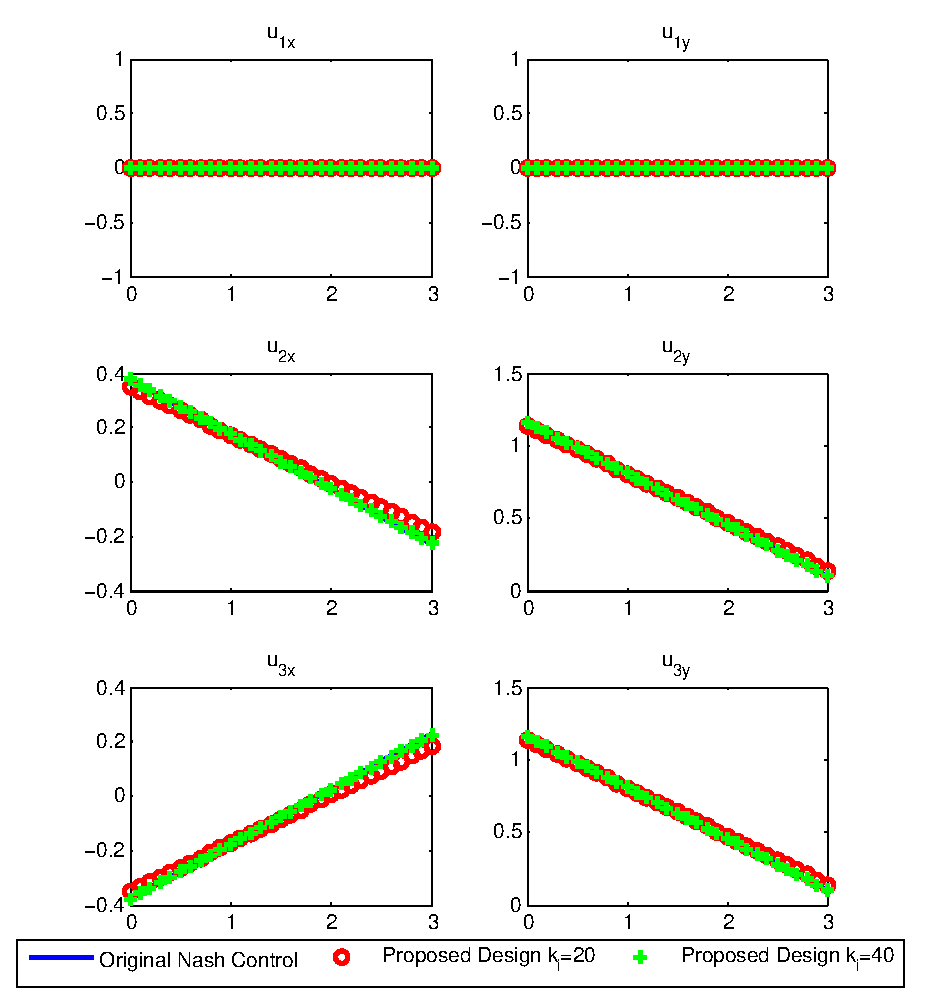
\includegraphics[scale=0.58]{Original_Distributed_control.eps}
      \caption{Nash and proposed designed strategies}\label{Original_Distributed_control}
\end{figure}
The motion trajectories under various control inputs are shown in Figure \ref{TrajectoryUndirected}.
\begin{figure}[h]
      \centering
      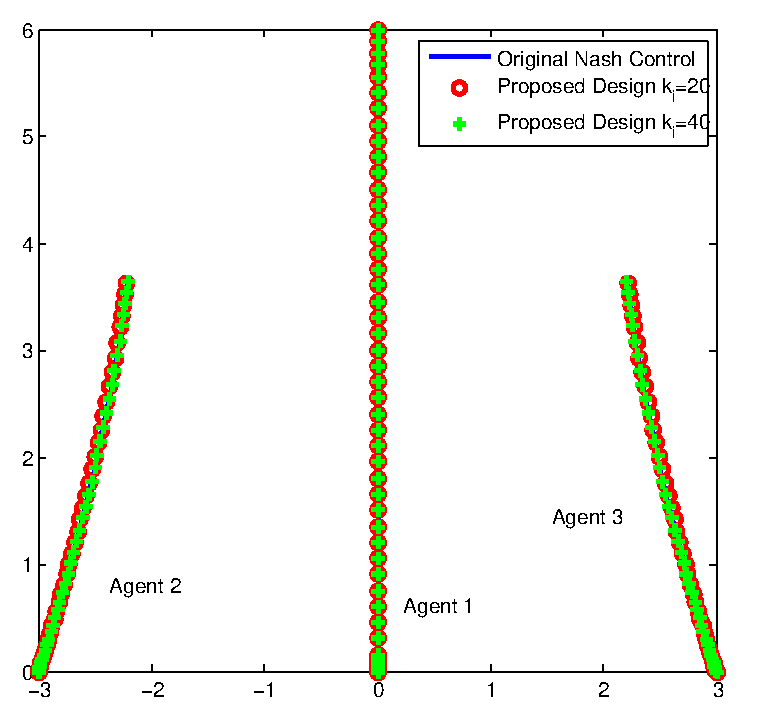
\includegraphics[scale=0.5]{TrajectoryUndirected.eps}
      \caption{Motion trajectories under different control strategies}\label{TrajectoryUndirected}
\end{figure}
Graphically, there does not exist much difference between the trajectories under the original Nash strategies and the ones under designed strategies. Quantitatively, we are able to calculate the total terminal formation error with respect to the desired displaced among the agents, which is
\begin{equation}
\eta=\sum^3_{i=1}\|s_1(t_f)-s_i(t_f)-{\mu_{1i}}\|,
\end{equation}
where $s_i(t_f)$ is agent $i$'s terminal position vector under certain control strategies. Therefore, the total terminal formation errors based on different values of $r_1=r_2=r_3=r$ and $k_1=k_2=k_3=k$ can be summarized into Table \ref{Comparison}.
\begin{table}[h]\normalsize
\centering
\begin{tabular}{|l|c|c|c|}
  \hline
  % after \\: \hline or \cline{col1-col2} \cline{col3-col4} ...
         & Nash & $k=20$ & $k=40$ \\
         \hline
         $\eta\;\;(r=0.2)$ & 0.2162 & 0.2177 & 0.2162 \\
         \hline
  $\eta\;\;(r=1)$ &  0.8164 &  0.8513 & 0.8179 \\
  \hline
  $\eta\;\;(r=5)$ &  2.6541 & 2.6920 & 2.6560 \\
  \hline
\end{tabular}
\caption{Total terminal formation errors in Scenario 1}\label{Comparison}
\end{table}
From the table, it is clear to see that the total terminal formation error decreases as $k_i$ increase because as mentioned, larger $k_i$ will result in more accurate terminal state estimates and more accurate control inputs (with respect to the Nash strategies). It is also clear to see that the total terminal formation error increases as $r$ increases. This is because that if agents put higher penalties on the control effort or energy (i.e., the quadratic term of the control input in (\ref{JiFormation})), they will try to reduce more on control energy instead of the terminal formation errors in order to minimize their performance indices in (\ref{JiFormation}) during the time period of the formation control. Based on more simulation data, the relationship among $\eta$, $k$, and $r$ can be depicted in Figure \ref{Relationship}.
\begin{figure}[h]
      \centering
      \includegraphics[scale=0.5]{PlotT.eps}
      \caption{Relationship among $\eta$, $r$, and $k$}\label{Relationship}
\end{figure}
As we can see in the figure, when $r$ is small, the variance of the total terminal formation error $\eta$ among different $k$ is small, and when $r$ is large, the variance of the total terminal formation error $\eta$ among different $k$ becomes large. Another application of Figure \ref{Relationship} is to determine the lowest update gain $k$ needs to achieve a desired terminal formation error. For instance, if we want to determine a update gain that can achieve a maximum terminal formation error of 2 given $r=2$, then we can find that a value of $k$ less than $6$ is good choice from the figure. Therefore, this figure provides a intuitive way of choosing a proper update gain, especially to avoid choosing a high gain which is undesired in many real life applications.

\textbf{Scenario 2}: We now consider the scenario where there are three agents with undirected communication topology as shown in Figure \ref{Formation3undirected}.
\begin{figure}[h]
      \centering
      \includegraphics[scale=0.8]{Formation3undirected.eps}
      \caption{Three agents with undirected graph}\label{Formation3undirected}
\end{figure}
With this communication topology, both Nash and Pareto strategies can be derived. The initial states of the agents and the performance index parameters are the same as the ones in Scenario 1. For both Nash strategy design and Pareto strategy design, the gain $k_i$ in the terminal state estimation equation (\ref{update}) and (\ref{updatehphv}) are set equal to $40$ for all $i=1,2,3$. For the Pareto strategies, the convex parameters in (\ref{convexcombination}) are set to be $\alpha_1=\alpha_2=\alpha_3=1/3$. The Laplacian matrix for the noncooperative in (\ref{laplacian}) and the one for the cooperative case in (\ref{laplacianFormation}) are
\[\mathcal{L}=\begin{bmatrix}
2&-1&-1\\
-1&1&0\\
-1&0&1
\end{bmatrix}\quad\mbox{and}\quad \mathcal{L}=\begin{bmatrix}
\frac{4}{3}&-\frac{2}{3}&-\frac{2}{3}\\
-\frac{2}{3}&\frac{2}{3}&0\\
-\frac{2}{3}&0&\frac{2}{3}
\end{bmatrix},\]
respectively. The resulting motion trajectories under both Nash and Pareto strategies are shown in Figure \ref{NashPareto}.
\begin{figure}[h!]
      \centering
      \includegraphics[scale=0.5]{NashPareto.eps}
      \caption{Motion trajectories under Nash and Pareto strategies}
      \label{NashPareto}
\end{figure}
The total terminal formation errors under different choices of the convex parameters are summarized in Table \ref{Scenario2Table}.
\begin{table}[h]\normalsize
\centering
\begin{tabular}{|c|c|}
  \hline
  % after \\: \hline or \cline{col1-col2} \cline{col3-col4} ...
       & $\eta$  \\
       \hline
  Nash & 0.4856  \\
  \hline
  Pareto ($\alpha_1=\alpha_2=\alpha_3=1/3$)&0.3033\\
  \hline
  Pareto ($\alpha_1=1/6,\alpha_2=2/3,\alpha_3=1/6$)&0.3128\\
  \hline
  Pareto ($\alpha_1=2/3,\alpha_2=1/6,\alpha_3=1/6$)&0.1791\\
  \hline
  Pareto ($\alpha_1=0.9,\alpha_2=0.05,\alpha_3=0.05$)&0.0602\\
  \hline
\end{tabular}
\caption{Total terminal formation errors in Scenario 2}\label{Scenario2Table}
\end{table}
As we can clearly see in the table, the agents can actually achieve lower formation error using Pareto strategies than using Nash strategies. This is because the agents are assumed to cooperate with each other in the Pareto optimality. Also note that as we place more weight on agent $1$'s performance index, the total formation error can be reduced. This is because it is much easier to move agent 1 alone to form the desired formation {instead} of moving all the three agents together.
%%%%%%%%%%%%%%%%%%%%%%%%%%%%%%%%%%%%%%%%%%%%%%%%%%%%%%%%%%%%%%%%%%%%%%%%%%%%%%%%

\section{Conclusion}\label{conclusion}
{This paper considers the design of open-loop Nash and Pareto strategies for multi-agent formation control problems. The proposed approach utilizes the distributed estimation of the terminal state variables among the agents through network-based information exchange. The convergence rate of the terminal state estimation algorithm is determined by a scalar gain and can be made sufficiently fast to get a better approximation of the real Nash and Pareto strategies. An illustrative example is solved with two scenarios and various comparisons have been made.}

%\addtolength{\textheight}{-12cm}% This command serves to balance the column lengths
                                  % on the last page of the document manually. It shortens
                                  % the textheight of the last page by a suitable amount.
                                  % This command does not take effect until the next page
                                  % so it should come on the page before the last. Make
                                  % sure that you do not shorten the textheight too much.
%
%Appendixes should appear before the acknowledgment.

%\section*{ACKNOWLEDGMENT}


\bibliographystyle{IEEEtran}
\bibliography{Mybib}




\end{document}
